\documentclass[11pt,twocolumn,twoside]{opticajnl}
%% Please use 11pt if submitting to AOP
% \documentclass[11pt,twocolumn,twoside]{opticajnl}

\journal{pr} % Choose journal (ao,jocn,josaa,josab,ol,optica,pr)

%See template introduciton for guidance on setting shortarticle option
\setboolean{shortarticle}{True}
% true = letter/tutorial
% false = research/review article
% (depending on journal)
\usepackage{lineno}
\usepackage[utf8]{inputenc}
\spanishdecimal{.}
\usepackage{amsmath}
\usepackage{caption}
\usepackage{subcaption}
\usepackage[spanish]{babel}
\usepackage{hyperref}
\usepackage{listings}
\usepackage{multicol}
\usepackage[export]{adjustbox}
%\linenumbers
\lstdefinestyle{mystyle}{
    language=Python, % Choose the programming language (e.g., Python)
    basicstyle=\ttfamily, % Set the font style
    keywordstyle=\color{blue}, % Define the color for keywords
    commentstyle=\color{green!40!black}, % Define the color for comments
    numbers=left, % Show line numbers
    numberstyle=\tiny, % Set the style for line numbers
    frame=single, % Add a frame around the code
    breaklines=true, % Allow line breaks within code
    showstringspaces=false % Don't show spaces within strings
}


% Configura el formato del título del listado
\renewcommand\lstlistingname{Código}
\renewcommand\lstlistlistingname{Códigos}
\title{
\vspace{0.1cm} 

Trabajo práctico 5: Memorias asociativas}

\author[1]{\huge{Ignacio Lembo Ferrari}}
\affil[1]{\large{ignaciolembo@ib.edu.ar} 

\vspace{0.1cm}

{\datesfont 17 de noviembre del 2023.}

\vspace{0.1cm}
}

%\begin{abstract}
%\textbf{hola}
%\end{abstract}

\begin{document}

\maketitle

\section{Modelo de Hopfield sin ruido \label{sec:ej1}}

\vspace{0.3cm}

Se utilizó una red de Hopfield sin ruido para resolver el problema de memorizar patrones. Para esto se crearon $p$ patrones con $N$ neuronas cada uno, $x_i^\mu$ $(i = 1,... N, \mu= 1,...,p)$, donde cada neurona $i$ puede tomar valores $\pm 1$ con igual probabilidad. A partir de estos patrones se calculó la matriz de conexiones mediante la regla de aprendizaje de Hebb
\begin{equation}
    w_{ij} = \frac{1}{N} \sum_{\mu=1}^p x_i^\mu x_j^\mu ~~~\forall ~~~ i \neq j, ~~~~~~~ w_{ii} = 0.
\end{equation}

Sea $s$ un estado con $N$ neuronas. En este modelo con dinámica determinista, se determina la evolución de la neurona $i$-ésima del estado $s$ con la siguiente regla
\begin{equation}
    s_i(t + 1) = \text{sgn} \left( \sum_{j=1}^N w_{ij} s_j(t) \right).
\end{equation}


En este punto existen dos maneras de actualizar el vector de neuronas, de forma secuencial o paralela. En el primer caso, se actualiza neurona por neurona de manera que la neurona $i$-ésima (con $i>0$) se actualiza con información de neuronas ya actualizadas. En el segundo caso, se calculan todos los $h_i(t)$ y luego se actualizan todas las neuronas al mismo tiempo y solo dependen de la información de neuronas en la iteración anterior. 
Luego, se deja evolucionar al sistema, tanto con dinámica secuencial o paralela hasta que el estado $s$ converja, es decir, $s(t+1) = s(t)$. En el caso de no darse la condición de convergencia se repite todo el proceso de actualización de las $N$ neuronas para todo el estado $s$. Se tomó cada patrón $\mu$ como condición inicial, es decir, $x_i^\mu = s(0)$.

En el caso de converger, se puede calcular el overlap $m^\mu$ para cada patrón $\mu$ como  
\begin{equation}
    m^\mu = \frac{1}{N} \sum_{i=1}^N x_i^\mu s_i^\mu.
\end{equation}
Veamos que las neuronas solo pueden tomar valores $\pm 1$, el overlap será $1$ en el caso que todas las neuronas en $s(t)$ coincidan con el patrón $x^\mu$. En este caso, la red reconoce perfectamente el patrón. Valores de overlap menores a $1$ implican que la red tiene problemas para reconocer el patrón. 

Este estudio se realizó para $N=500,1000,2000,4000$ neuronas y $\alpha = 0.12,0.14,0.16,0.18$ donde $p = N\alpha$ es el número de patrones. Esto se realizó tanto para la dinámica secuencial como paralela. En el caso de la dinámica paralela no se obtuvo convergencía de los estados $s$. Por otra parte, en la dinámica secuencial, sí se obtuvo convergencia. En la Fig. \ref{fig:hist_sec}  se muestran los histogramas para todos los estudios realizados. Se observa que para $\alpha = 0.12, 0.14$ la distribución del overlap es unimodal entorno a $1$ para todo $N$. Al aumentar $\alpha$ el reconocimento de la red empeora y se observa que el overlap se distribuye en forma bimodal torno a $m = 1$ y $m \approx 0.3$. Para estos últimos casos de $\alpha$ grande se obtiene una distribución bimodal donde al aumentar $N$ se observan cada vez más valores entorno a $m \approx 0.3$. En el caso particular, de $N$ y $\alpha$ máximos se observa una distribución unimodal en torno a $m \approx 0.3$.


\begin{figure*}[t]
    \centering
        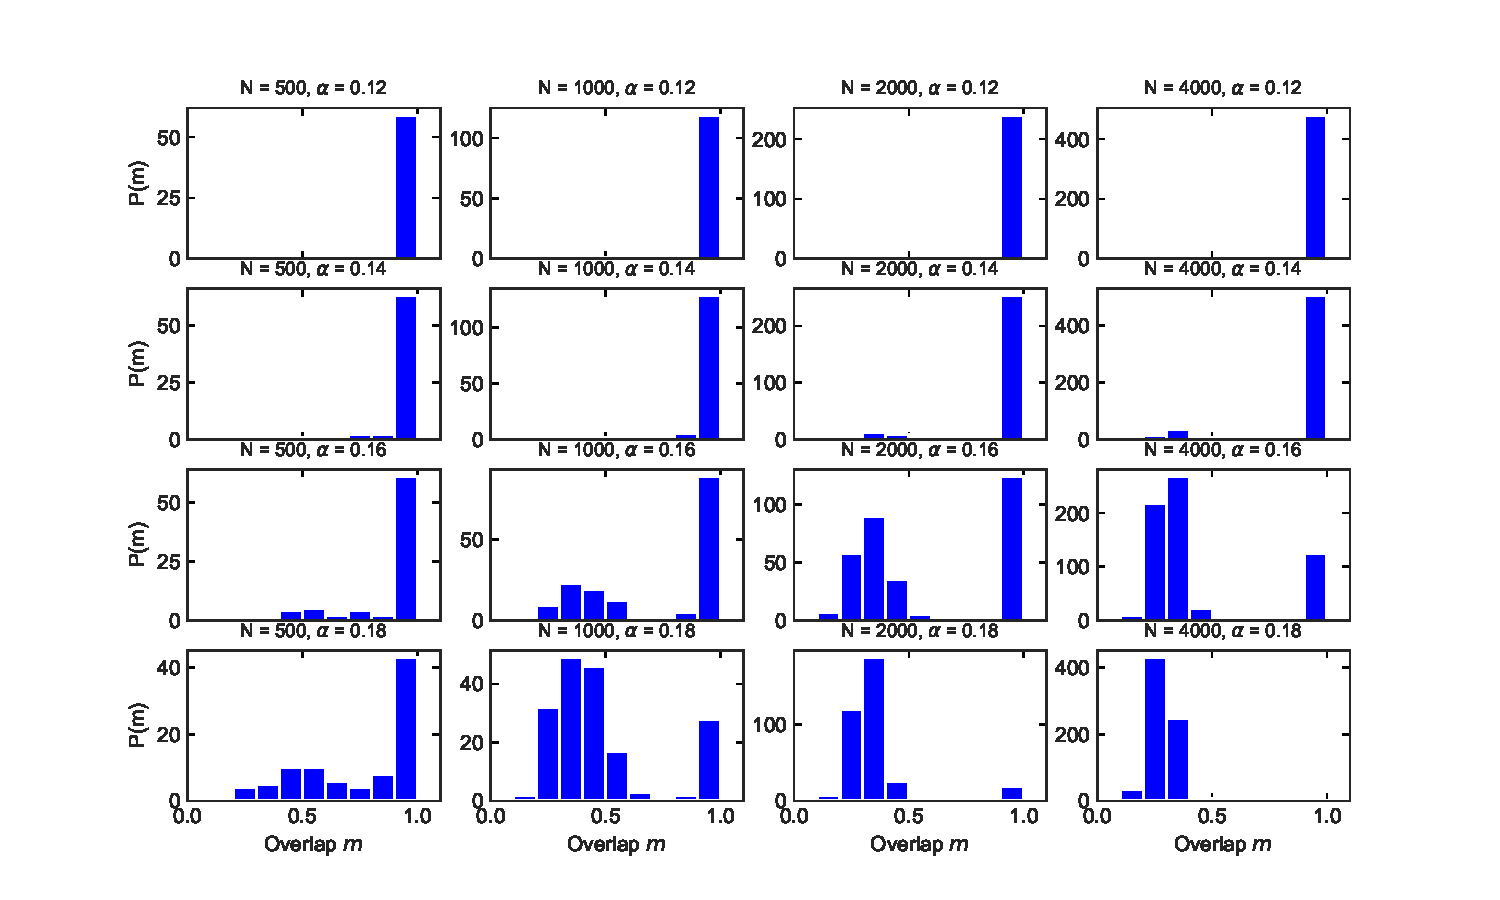
\includegraphics[width=\textwidth]{Figuras/hist_sec.pdf}
    \caption{Distribución del overlap $m$ para una red de Hopfield sin ruido con dinámica secuencial entrenada con $p$ patrones. Se muestran estudios para $N=500,1000,2000,4000$ y $\alpha = 0.12,0.14,0.16,0.18$ donde $N$ es el número de neuronas por patrón y $p = N\alpha$ el número de patrones.} 
    \label{fig:hist_sec}
\end{figure*}


\section{Modelo de Hopfield con ruido\label{sec:ej2}}

\vspace{0.3cm}

Se simuló la dinámica de Hopfield con ruido. En este caso, a diferencia de la sección anterior, la ley que actualiza las neuronas $s_i(t)$ a tiempo $t$ está dada de forma estocástica por
\begin{equation}
    P_r(s_i(t+1) = \pm 1) = \frac{\text{exp}(\pm \beta h_i(t))}{\text{exp}(\beta h_i(t)) + \text{exp}(- \beta h_i(t))}.
\end{equation}
donde $\beta = 1/T$ y $h_i(t) = \sum_{j=1}^N w_{ij} s_j(t)$. 

Al igual que antes se tomó cada patrón como condición inicial, $x_i^\mu = s(0)$. Se dejó evolucionar al sistema recorriendo las $N$ neuronas de forma secuencial hasta recorrer un total de 10 veces cada neurona.

\newpage

En la Fig. \ref{fig:m_vs_T} se muestra el overlap promedio $\overline{m}$ en función de la temperatura $T$ para una red de Hopfield con ruido con dinámica secuencial entrenada con $p=40$ patrones y $N=4000$ neuronas cada uno. Se grafican además la franja de incerteza dada por el desvío estándar de los valores de $m$. 
En primer lugar, se observa una temperatura crítica cerca de $T = 1.0$ donde el overlap pasa de 1 a 0. lo cual es esperado para $p \ll N$. Se observa que para valores bajos de $T$ el error cuadrático medio es bajo y se agranda a medida que aumenta $T$, luego de la transición este error se mantiene aproximadamente constante. A $T$ pequeño entonces vemos que la red reconoce bien los patrones ya que el overlap es $1$ y luego de la transición a $T=1.0$ la red deja de reconocer los patrones y el overlap se va a $0$. 

\centerline{\rule{0.95\linewidth}{0.6pt}}

\begin{figure}[H]
    \centering
    \begin{subfigure}[h]{\linewidth}
        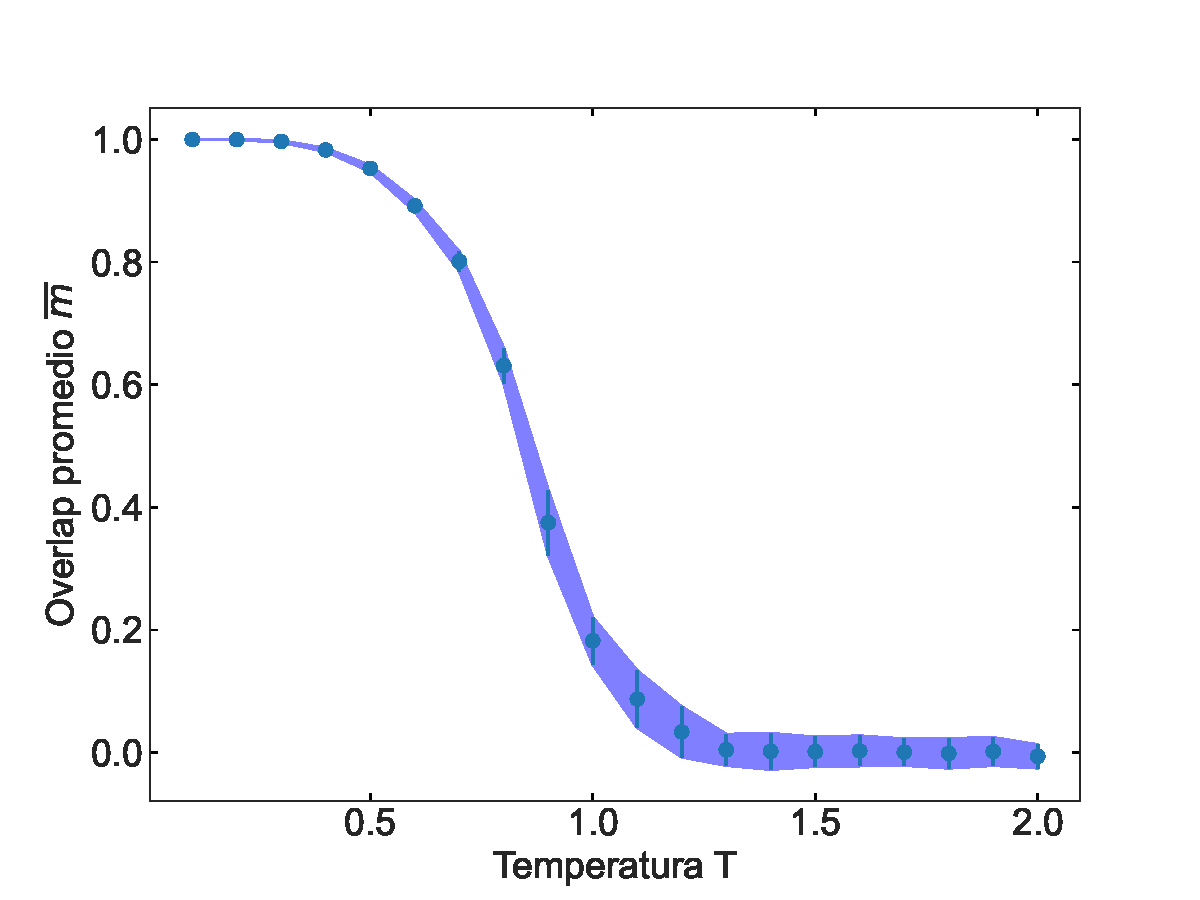
\includegraphics[width=\textwidth]{Figuras/m_vs_T.pdf}
     \end{subfigure}
    \caption{Overlap promedio $\overline{m}$ en función de la temperatura $T$ para una red de Hopfield con ruido con dinámica secuencial entrenada con $p$ patrones. Se utilizaron $p=40$ patrones con $N=4000$ neuronas cada uno. Se grafican además la franja de incerteza dada por el desvío estandar de los valores de $m$.} 
    \label{fig:m_vs_T}
\end{figure}








% Bibliography
%\renewcommand*{\bibfont}{\normalsize}
%\bibliography{Redes}

% Full bibliography added automatically for Optics Letters submissions; the following line will simply be ignored if submitting to other journals.
% Note that this extra page will not count against page length
%\bibliographyfullrefs{Redes}

\clearpage

\begin{onecolumn} % Activa una sola columna para el apéndice
\appendix
\section{Apéndice \label{codigo}}

\scriptsize
\subsection{Ejercicio 1}
\begin{lstlisting}[style=mystyle]
    import numpy as np
    import matplotlib.pyplot as plt
    from tqdm import tqdm
    import random
    
    #Ploteo 
    import seaborn as sns
    #sns.axes_style("whitegrid")
    sns.set_style("ticks")
    
    def genera_patrones(p, N):
        return np.array([[random.choice([-1, 1]) for _ in range(N)] for _ in range(p)])
    
    Ns = [500,1000,2000,4000]
    alphas = [0.12,0.14, 0.16, 0.18]
    
    fig, axs = plt.subplots(nrows=len(alphas), ncols=len(Ns), figsize=(10, 6))
    
    j = 0
    for N in Ns:
        idx = np.arange(N)
        l = 0
        for alpha in alphas:
    
            #Generacion de patrones
            x = genera_patrones(int(N*alpha), N)
            #Matriz de conexiones
            w = np.zeros((N,N))
            #Vector de overlaps
            m = np.zeros(int(alpha*N))
    
            for u in range(int(alpha*N)):
                w += (1/N)*np.dot(x[u].reshape(-1,1), x[u].reshape(1,-1))
            np.fill_diagonal(w, 0)
    
            #Secuencial
            print("Secuencial - N=", N, " - alpha=", alpha) 
            for u in tqdm(range(int(alpha*N))):
                s = x[u].copy()
                f = True
                while f:
                    r = 0 
                    #np.random.shuffle(idx)
                    f = False
                    for i in idx:
                        h = np.sign(np.dot(w[i], s))
                        if(s[i]*h < 0):
                            f = True
                        s[i] = h
                    #if(r==1000):
                    #    f = False
                    #    print("Corto por limite de iteraciones")
                    #r += 1
    
                #overlap
                m[u] = (1/N)*np.dot(x[u],s)
    
            bin_width = 0.1  # Ancho constante de los bins
            bin_edges = np.arange(0, 1 + bin_width, bin_width)
            axs[l,j].hist(m, bins=bin_edges, alpha=1, color='b')
            axs[l,j].set_title(f"N = {N}, $\\alpha$ = {alpha}", fontsize = 9)
            axs[l,j].tick_params(direction='in', top=True, right=True, left=True, bottom=True)
            axs[l,j].tick_params(axis='x', rotation=0, labelsize=10, color='black')
            axs[l,j].tick_params(axis='y', labelsize=10, color='black')
            axs[l,j].set_xlim(0, 1.1)
            if(l != len(Ns)-1 ):
                axs[l,j].axes.xaxis.set_ticklabels([])
            #if(j != 0):
                #axs[l,j].axes.yaxis.set_ticklabels([])
        
            """
            #Paralelo
            m = np.zeros(int(alpha*N))
            print("Paralelo - N=", N, " - alpha=", alpha)
            for u in tqdm(range(int(alpha*N))):
                s_j = x[u].copy()
                s_i = s_j.copy()
                f = True 
                idx = 0
                while f:
                    s_i = np.sign(np.dot(w, s_j.reshape(-1,1)))
                    if((s_i == s_j).all() or idx == 1000):
                        f = False
                    s_j = s_i
                    idx += 1    
                print("Alcanzo el limite de iteraciones")
            """
            l = l + 1
        j = j + 1 
    
    for j in range(len(Ns)):
        axs[len(Ns)-1,j].set_xlabel("Overlap $m$")
    for l in range(len(alphas)):
        axs[l,0].set_ylabel("P(m)")
    
    fig.savefig(f"../Redes-Neuronales/Practica_6/resultados/ej1/hist_sec.pdf")
    fig.savefig(f"../Redes-Neuronales/Practica_6/resultados/ej1/hist_sec.png", dpi=600)
    plt.show()
\end{lstlisting}
\subsection{Ejercicio 2}
\begin{lstlisting}[style=mystyle]
    import numpy as np
    import matplotlib.pyplot as plt
    from tqdm import tqdm
    import random
    
    #Ploteo 
    import seaborn as sns
    #sns.axes_style("whitegrid")
    sns.set_style("ticks")
    
    def genera_patrones(p, N):
        return np.array([[random.choice([-1, 1]) for _ in range(N)] for _ in range(p)])
    
    def signo_T(h, T):
        p = np.exp(h/T) / (np.exp(h/T)+np.exp(-h/T))
        q = 1 - p
        s = np.random.choice([1, -1], p=[p, q])
        return s
    
    N = 4000
    p = 40
    Ts = np.arange(0.1, 2.1, 0.1)
    its = 10
    
    #Vector de overlaps
    m_p = np.zeros(len(Ts))
    m_std = np.zeros(len(Ts))
    fig1, ax1 = plt.subplots(figsize=(8,6))
    
    #Generacion de patrones
    x = genera_patrones(p, N)
    #Matriz de conexiones
    w = np.zeros((N,N))
    for u in range(p):
        w += (1/N)*np.dot(x[u].reshape(-1,1), x[u].reshape(1,-1))
    np.fill_diagonal(w, 0)
    
    t = 0
    idx = np.arange(N)
    for T in tqdm(Ts):
        m = np.zeros(p)
        for u in range(p):
            s = x[u].copy()
            for it in range(its):
                ##np.random.shuffle(idx)
                for i in idx:
                    h = np.dot(w[i,:], s)
                    s[i] = signo_T(h, T)
            #overlap
            m[u] = (1/N)*np.dot(s,x[u])
        m_p[t] = np.mean(m)
        m_std[t] = np.std(m)
        t += 1
    
    ax1.errorbar(Ts, m_p, yerr=m_std, fmt='o')
    ax1.fill_between(Ts, m_p+m_std, m_p-m_std, alpha=0.5, color="blue")
    ax1.set_xlabel(r"Temperatura T", fontsize=18)
    ax1.set_ylabel(r"Overlap promedio $\overline{m}$", fontsize=18)
    ax1.tick_params(direction='in', top=True, right=True, left=True, bottom=True)
    ax1.tick_params(axis='x', rotation=0, labelsize=18, color='black')
    ax1.tick_params(axis='y', labelsize=18, color='black')
    
    fig1.savefig(f"../Redes-Neuronales/Practica_6/resultados/ej2/m_vs_T.pdf")
    fig1.savefig(f"../Redes-Neuronales/Practica_6/resultados/ej2/m_vs_T.png", dpi=600)
    
    plt.show()
\end{lstlisting}
\end{onecolumn}
\end{document}


